%************************************************
\chapter{Background on Event-Driven Business Process Management}\label{ch:background}
%************************************************

\section{Business Process Management}\label{ch:bg:bpm}
With its origins dating back to the process orientation trend of the 1990s, \ac{BPM} has meanwhile become a mainstream tool to support organizations.
It had been noted, that company workflows can essentially be broken down into activities that are executed in a coordinated manner by one or more parties.
A certain group of activities thereby form a process which is executed within an organization.
More precisely, \citeauthor{weske:bpm-book} \cite{weske:bpm-book} defines a single \emph{business process} as follows:

\begin{description}
	\item[Definition 1 (Business Process):]
	A \emph{business process} consists of a set of activities that are performed in coordination to realize a business goal. Each business process is enacted by a single organization, but it may interact with processes performed by other organizations.
\end{description}

\noindent The term \emph{Business process management} describes the techniques available to develop and support processes throughout their life-cycle.
It is grounded in the use of explicit process representations which ultimately allow the exchange, analysis and reproduction of the workflows.
This process specification is referred to as the \emph{business process model}, composed mainly of activities and the rules that are necessary to coordinate their execution.
When a process is performed according to its model, the single execution is called \textit{process instance}.
Based on a process model, the number of possible instances is theoretically unbounded.

\begin{description}
	\item[Definition 2 (Business Process Model):]
	A \emph{business process model} consists of a set of activity models and execution constraints between them. A \emph{business process instance} represents a concrete case in the operational business of a company, consisting of activity instances.
	\cite[p.~7]{weske:bpm-book}
\end{description}

\noindent
The lifecycle of a business process can be  described in four cyclic phases in that numerous stakeholders interact and contribute depending on their specialization.
Process development starts with a \emph{Design \& Analysis} phase which yields a refined and validated business process model.
In the following \emph{Configuration} phase, it is necessary to prepare the process implementation, select the means and an environment to run the process in.
The action of making the process runnable in the execution environment is called \emph{process deployment}.
After these preparations the process can be enacted in daily business while its current state is monitored and system maintenance is performed if necessary (\emph{Enactment} phase). 
A single process execution begins with the \emph{process instantiation}, when the process has succeeded or is aborted, we say the process is \emph{terminated}.
During the enactment, system and stakeholders can start collecting performance indicators and process execution logs to allow evaluating the quality of the process specification. If that \emph{Evaluation} step reveals deficiencies, the lifecycle starts over by re-entering the design phase.
The \emph{process un-deployment} is performed if necessary, so that no new instances of the process can be started.
\cite[p.~11~ff.]{weske:bpm-book}
\todo[inline]{add reference to \cite{dumas:bpm}, mention that Weske says pretty much the same}
%the investigations undertaken in this work target the Design \& Analysis phase

\subsection{Business Process Meta Model and Activity Lifecycle}\label{ch:bg:bpmetamodel}
Attempting to...

\begin{description}
	\item[Definition 3 (Business Process Meta Model):]
	Let $C$ be a set of control flow constructs. $P = (N,E,type)$ is a \textit{process model} if it consists of a set $N$ of nodes, and a set $E$ of edges. \cite{weske:bpm-book},~p.~91
	\begin{itemize} 
		\item
		$N = N_{A}\cup N_{E}\cup N_{G}$, where $N_{A}$ is a set of activity models, $N_{E}$ is a set of event models and $N_{G}$ is a set of gateway models. These sets are mutually disjoint.
		\item 
		$E$ is a set of directed edges between nodes, such that $E\subseteq N \times N$, representing control flow.
		\item
		$type:N_{G}\rightarrow C$ assigns to each gateway model a control flow construct.
	\end{itemize}
\end{description}

\todo[inline]{
Much like the process instance lifecycle, each activity follows a cycle
- introduce activity lifecycle/control flow
}
\missingfigure{activity lifecycle}

%
While traditionally activities are executed manually by company staff following the written process specifications, computer systems are used today to drive the execution and enforcement of business processes and organizational rules.
The generic software systems utilized for that purpose are introduced in the following section.

\subsection{Business Process Management Systems}\label{ch:bg:bpms}
The implementation of business processes has developed from a manual execution guided by business rules to a fully automatized execution in a specialized IT environment.
One of the main reasons for \acs{BPM}'s growing popularity is that in today's fast-paced economy, a large part of the business activity is either supported by computers or even carried out autonomously by them.
The specialized software systems that are utilized to support the enactment of business processes are referred to as \emph{business process management systems}.

\paragraph{Process Management Architecture}
A typical IT infrastructure for driving business processes is illustrated in \autoref{fig:bpm-architecture}. 
Five principal building blocks are considered which will be explained in the following.

With reference to the business process lifecycle, the visualized scenario commences with the \emph{Business Process Modeling}. As a result of the \emph{Design \& Analysis} phase, new process models are created and refined to be stored in the \emph{Business Process Model Repository}. 
The relation between the two elements includes writing new models to the repository as well as reading models for review and further modification.
Given that the desired model is approved for enactment, the process gets deployed to the \emph{Process Engine} as part of the configuration step.
The process engine is the heart of the execution environment. It performs the execution of the processes from deployment until un-deployment, while the enactment and instantiation is controlled by the \emph{Business Process Environment}.
An indefinite number of \emph{Service Provider}s realize application services to support the process execution. A service provider can be a software module but also a knowledge worker performing a particular process step.

\begin{figure}[]
	\myfloatalign
	{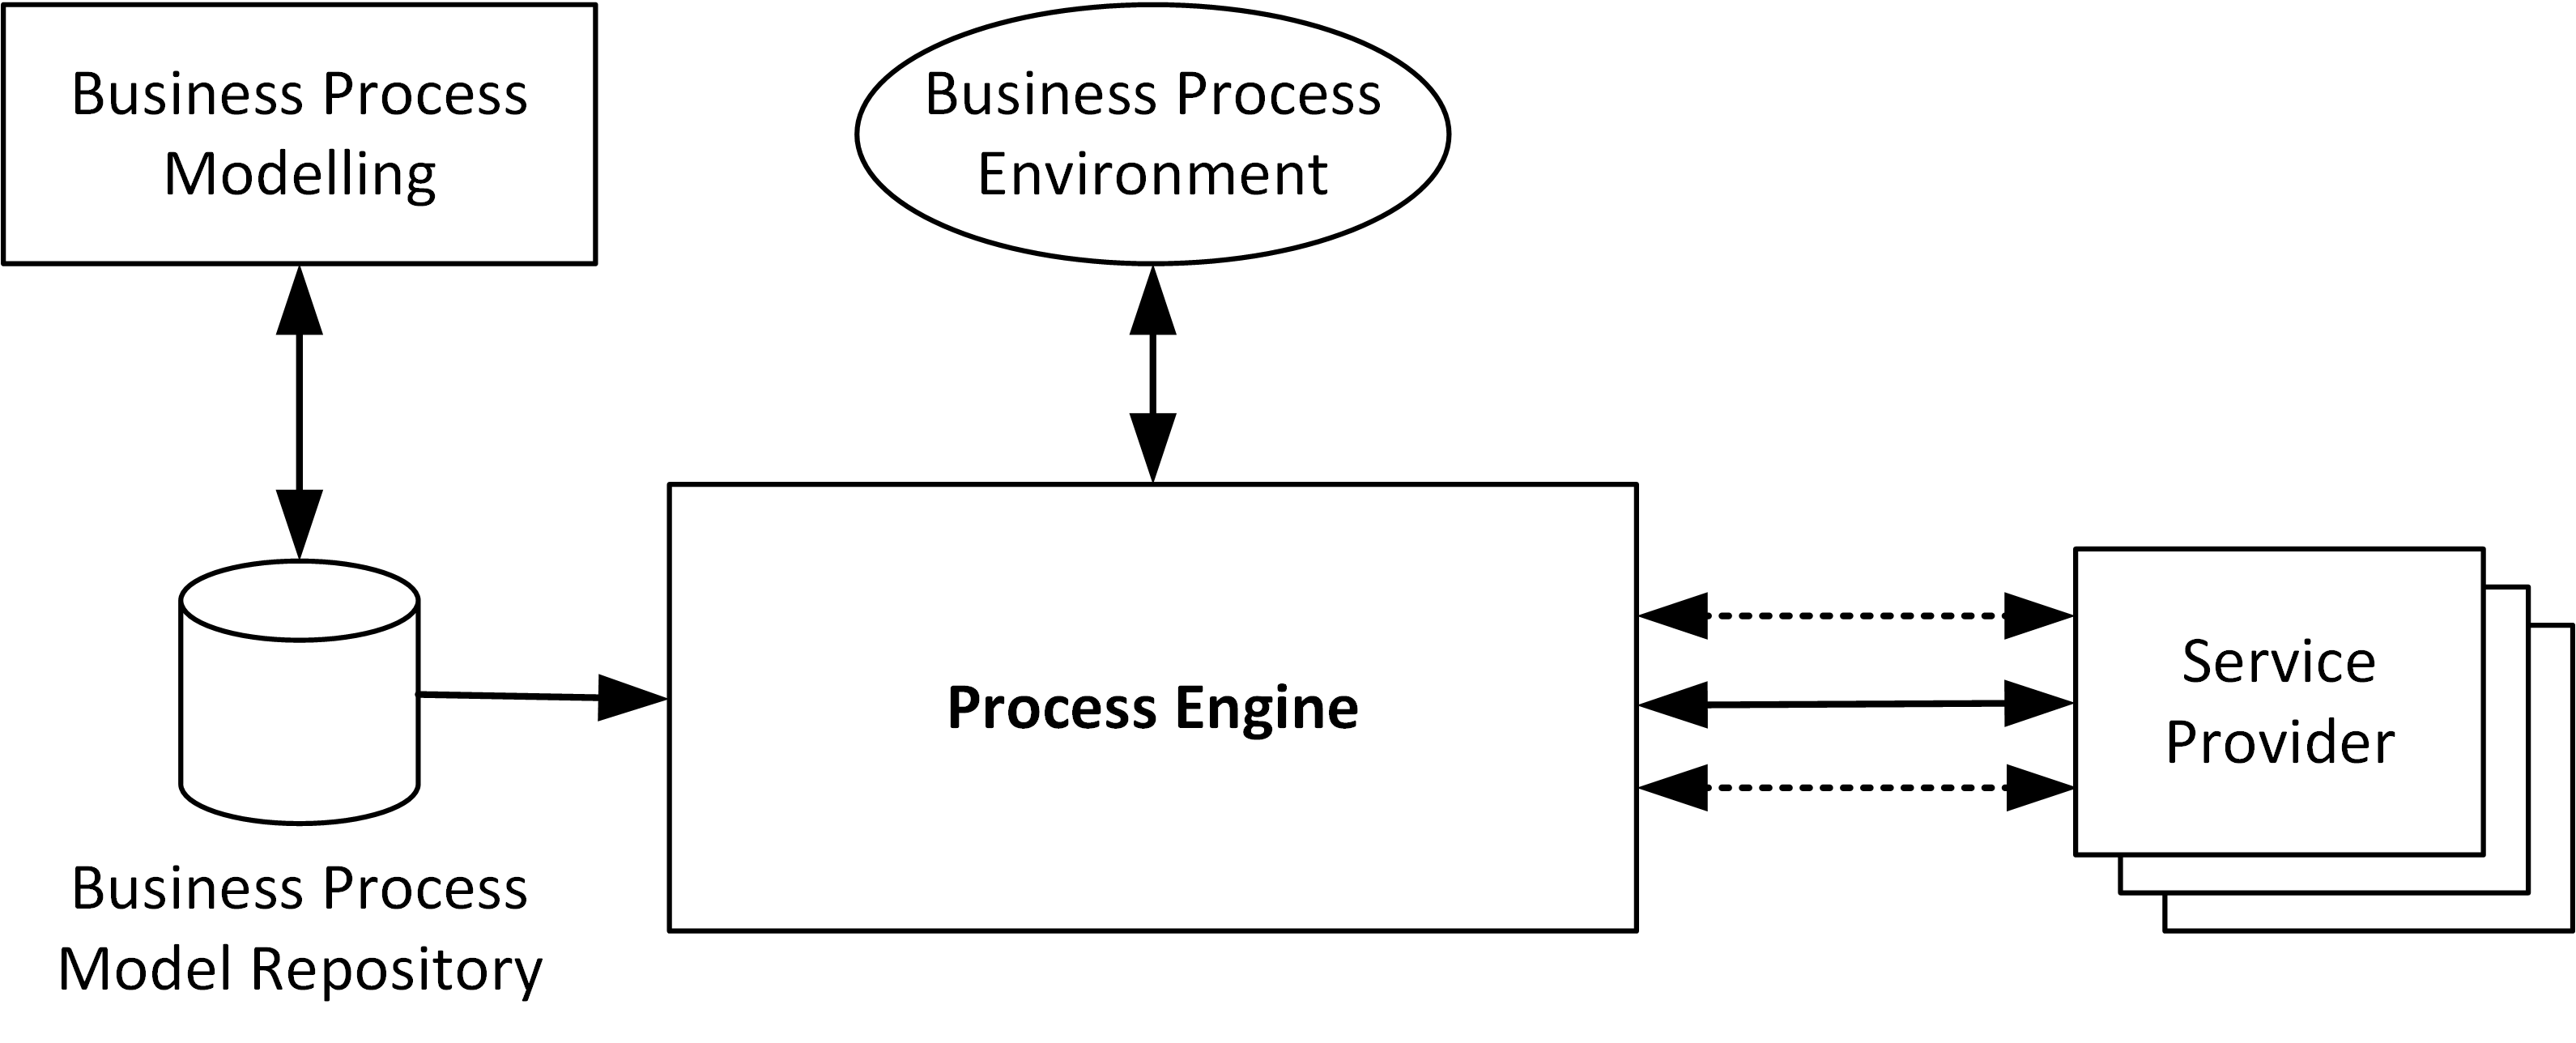
\includegraphics[width=1\linewidth]{chapters/background/bpm-architecture.png}}
	\caption{Business process management systems architecture model (see~\cite{weske:bpm-book},~p.~120)}
	\label{fig:bpm-architecture}
\end{figure}


\paragraph{The Camunda Business Process Engine}\label{ch:bg:camunda}
A large and ever growing number of process engines is available on the market, including solutions from IT giants like SAP, IBM and Oracle.
In this work, \emph{Camunda BPM}~\cite{camunda} has been chosen to illustrate implementations.
As of August 2017, the software product is available in version 7.7.0 and comes in a commercial, regularly updated version and in a free, community-driven solution that is updated with every major release.
Camunda is popular among the research community as the source code is openly available, the product is mature, but actively developed and offers comprehensive support for BPMN 2.0. It is designed to be extensible and easily modifiable to adapt to custom requirements.
\emph{Camunda BPM} comprises a modeling tool, the Camunda process engine core and a number of browser-based user-interfaces to control process enactment and monitor execution state.
\autoref{ch:implementation} will provide further details about the engine architecture and extension mechanisms.


\subsection{Business Process Model and Notation}
Given the general semantics of business processes, a specific modeling notation has to be selected to express an informal process description in a formal, interchangeable way.
Different languages and notations have become available over the years, each serving different specializations.
Kossak~et~al.~\cite{kossak:bpmn2} organize some of the more popular languages as follows: A subset of them are focused on the control flow of business processes, for instance \ac{BPMN}~\cite{bpmnspec}, Yet Another Workflow Language and Petri Nets; some focus on object-orientation, like \ac{UML} activity diagrams and use case diagrams; some are data-flow oriented, e.~g.~the Structured Analysis and Design Technique.
\todo[inline]{references to the other languages}

Among these, the \acs{BPMN} has developed into a widely-adopted industry standard, also becoming ISO-standard in 2013~\cite{iso2013bpmn}.
The standard is developed by the Object Management Group~\cite{omghome} and now available in version 2.0~(January~2011) after being first released in January~2008.
\acs{BPMN} can be understood as an extension to the abstract business process meta model~(\autoref{ch:bg:bpmetamodel}) adding a comprehensive catalog of visual representations and semantic constructs. Furthermore, one of the most important features of its latest version is the a standardized interchange format provided through an XML specification, as \cite{weske:bpm-book} points out.
As emphasized by \citeauthor{Muehlen:2007}~\cite{Muehlen:2007}, the increased expressiveness of modern languages like \acs{BPMN} comes at the cost of an increased complexity. An aspect that, apparently, did not stop it from gaining popularity.

\paragraph{Core Building Blocks of a BPMN Model}

Following the business process meta model, a \acs{BPMN} model is a node-edge-model whereas nodes are either \emph{Activity Models}, \emph{Event Models} or \emph{Gateway Models}.

- main elements:
-> briefly explain
- events: why? how?


\missingfigure{Sample BPMN model}
- explain what happens in that process

\paragraph{Process Choreographies}
- Message
- choreographies

\missingfigure{Sample BPMN model}


\section{Complex Event Processing}
- what does it do
- how does it generally work
-> stream processing and | input > processing > output |
- Event queries: Esper
- event producer, consumer, subscription
-> pub/sub; temporal order sub > occur > unsub

\missingfigure{pub/sub workflow}

\section{Events in Business Processes}
- there are 2 use cases for events in bp: (1) for process monitoring, (2) for driving processes
%Brandl H.-M. and Guschakowski D. Complex Event Processing in the Context of Business Activity Monitoring

- interplay BPT to CEP platforms, 
> sub in BPMN should rather be 'Problem Statement' somehow
- putting cep queries into bpmn models => heiko's thesis or other related work?
- how can events be used
- exercise through one example



